\section{Design of \TwoLevelIndex{}}
\label{index}

In this paper, we aim to solve \probdef{} problems with a novel \twolevelindex{}. We first describe the structure and construction of the \twolevelindex{}. Then we show how to process queries with it. \usernote{We show the flow chart of index construction and query process in \autoref{fig:flow}.}

\subsection{Construction of \TwoLevelIndex{}}

%\subsection{Overview}
The index proposed in this paper contains two levels to efficiently process both \toplevelprob{} queries and \bottomlevelprob{} queries. %The top level index provides information at the community level while the bottom level index offers information at the edge level. 
The top level is a super-graph, called \treeindex{}, whose vertices represent unique k-truss communities and edges represent the containment relations between k-truss communities. 
%One can easily locate relevant communities of a given query by using our $union-intersection$ operation (We will discuss $union-intersection$ operation in Section \ref{query}). 
The bottom level is a maximum spanning forest of a \inducedgraph{} that preserves the edge level trussness and triangle connectivity inside the k-truss communities. 
%After the relevant communities being retrieved, we can discover their inner community edge-level structures with the bottom level index instead of resorting to expensive triangle enumeration. An overview of the index is shown in \autoref{fig:illustration_main}. 

The index is constructed in a bottom-up manner. In the following, we first formally define the \inducedgraph{} and introduce the algorithm to construct it from the original graph (Section~\ref{bottom-level}). Then we introduce the \treeindex{} and show how to use simple graph traversals on the bottom-level index to create the \treeindex{} (Section~\ref{top-level}). 

\subsubsection{MST of \InducedGraph{}}
\label{bottom-level}
~\\The \inducedgraph{} of an original graph $G^o$ is obtained by associating a vertex with each edge of $G^o$ and connecting two vertices if the corresponding edges of $G^o$ belong to the same triangle. Then we only store a maximum spanning tree of the \inducedgraph{}, which is enough to store the edge-level structures of k-truss communities in the original graph. We show the formal definition of a \inducedgraph{} in \autoref{def:\inducedgraph{}}. We show an example of the \inducedgraph{} and its maximum spanning forest in \autoref{fig:\inducedgraph{}}. We outline the maximum spanning forest with bold lines. 

\begin{Def}[\inducedgraph{}]
The \inducedgraph{} $G^t$ is a weighted undirected graph where each edge in the original graph $G^o$ is represented as a vertex in $G^t$. $G^t$ has an edge $e^{t}$ which connect vertices $v^{t}_{1}, v^{t}_{2} \in G^{t}$ if and only if their corresponding edges $e^{o}_{1}, e^{o}_{2} \in G^{o}$ belong to the same triangle in $G^o$. The weight of a vertex in $G^{t}$ is defined as the trussness of its corresponding edge in $G^o$. The weight of an edge in $G^{t}$ is defined as the lowest trussness of edges in the corresponding triangle in $G^{o}$. Thus, the weight of an edge in $G^t$ is always smaller or equal to the weights of adjacent vertices.
\label{def:\inducedgraph{}}
\end{Def}

\begin{figure}[h]
    \centering
    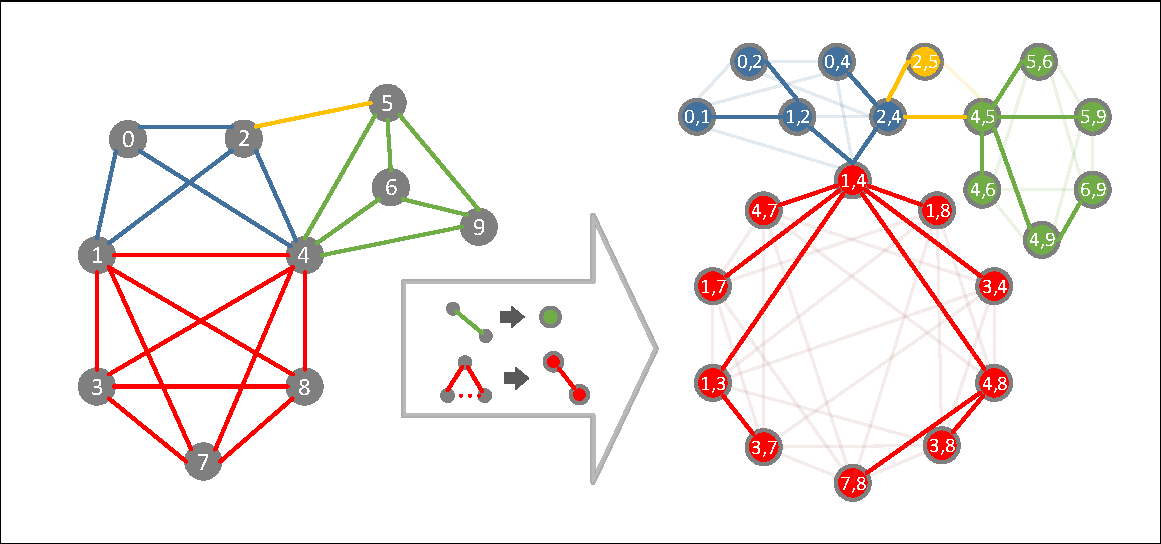
\includegraphics[width=0.8\linewidth, trim={0.8cm 0.6cm, 0.8cm, 0.6cm}, clip]{./figures/bottom_level.pdf}
		\vspace{-0.2cm}
    \caption{An example of the \inducedgraph{} and its maximum spanning tree of the example graph. We show the id of each vertex in the underlying graph on the left. We use a pair of ids of vertices in the underlying graph as the id of a vertex of the \inducedgraph{} on the right. }
    \label{fig:\inducedgraph{}}
		\vspace{-0.2cm}
\end{figure}

We use $G^m$ to denote the maximum spanning forest of $G^t$ that has been stored as the bottom-level index. To construct $G^m$, one way to do this is by generating the \inducedgraph{} $G^t$ first and then finding a maximum spanning tree of it. However, this approach is impractical because we need to sort the edges in $G^t$, which can be an order of magnitude larger than the origianl graph $G^o$. We use two methods to avoid this. First, we find that for real-world graphs, the highest edge trussness is usually small compared to the size of the graph, \eg only a few thousand for the densest graph in our experiments. Hence, we can use counting sort instead of comparison sort to reduce the time complexity. Second, since edge weight in $G^t$ represents the minimum edge trussness in the corresponding triangle in $G^o$, we can sort edges in the original graph $G^o$ to get the sorted order of the triangles in $G^o$ which can be translated to sorted order of edges in $G^t$. These two methods reduce both the time and space complexities of the maximum spanning tree algorithm.
%The details of the algorithm are shown in Algorithm \ref{alg:\inducedgraph{}_construction}. Note that the MAKE-SET operation makes a set contains only a single edge, and the FIND-SET operation returns the SET that contains a given edge.%\autoref{alg:\inducedgraph{}_construction}. 

%Since only $G^m$ will be stored in the bottom level index, we will refer to $G^m$ as the \inducedgraph{} in the following of the paper for similicity.

%\begin{algorithm}
	%\KwData{$G^{o}(V^{o},E^{o})$, edge trussness $\{\tau_{e}, e \in E^{o}\}$}
	%\KwResult{The \inducedgraph{} $G^{m}(V^{m}, E^{m})$}
	%\BlankLine
	%$sorted \gets$ sort edge trussness in decreasing order\;
	%\For{$e \in E^{o}$} {
	   %$V^{m} \gets V^{m} \bigcup \{e, \tau_{e}\}$\;
		 %MAKE-SET($e$)\;
	%}
	%\For{$(u,v) \in sorted$}{
		%suppose $u$ is the lower degree end of $(u,v)$\;
		%\For{$w \in N_{u}$}{
			 %\If{$(v,w) \in E^{o}$ \textbf{and} $\tau_{u,v} < \tau_{u,w}$ \textbf{and} $\tau_{u,v} < \tau_{v,w}$}{ 
				%\Comment{Compare edge id if trussness of edges are equal to avoid duplication.}\;
				%$\tau_{\triangle} = min(\tau_{(u,v)}, \tau_{(u,w)}, \tau_{(v,w)})$\;
				%% $E^{\triangle} \gets \{((u,v),(u,w)), \tau_{\triangle}\} \bigcup \{((u,v),(v,w)), \tau_{\triangle}\} \bigcup \{((u,w),(v,w)), \tau_{\triangle}\}$\;
				%$E^{\triangle} \gets \triangle_{u,v,w}$\;
				%\For{$e^{\triangle} \in E^{\triangle}$}{
				  %\If{FIND-SET($e^{\triangle}.v_1$) $\neq$ FIND-SET($e^{\triangle}.v_2$)}{
						%$E^{m} \gets E^{m} \bigcup e^{\triangle}$\;
						%UNION($e^{\triangle}.v_1$, $e^{\triangle}.v_2$)\;
					%}
				%}
			%}
		%}
	%}
	%\Return{$G^{m}(V^{m},E^{m})$}
	%\caption{Bottom Level Index Construction}\label{alg:\inducedgraph{}_construction}
%\end{algorithm}
We need edge trussness before constructing bottom-level index, which can be computed using the truss decomposition algorithm \cite{wang2012truss}, as inputs. The time and space complexities for constructing the bottom-level index are dominated by the computation of edge trussness of $G^o$, which are $O(\sum_{(u,v) \in E^{o}}{min\{d_{u},d_{v}\}})$ and $O(|E^{o}|)$,  respectively. Since $G^m$ is a maximum spanning forest, the bottom-level index takes $O(|V^{m}|) = O(|E^{o}|)$ space to store it.

\subsubsection{\TreeIndex{}}
\label{top-level}

\begin{figure}[h]
    \centering
    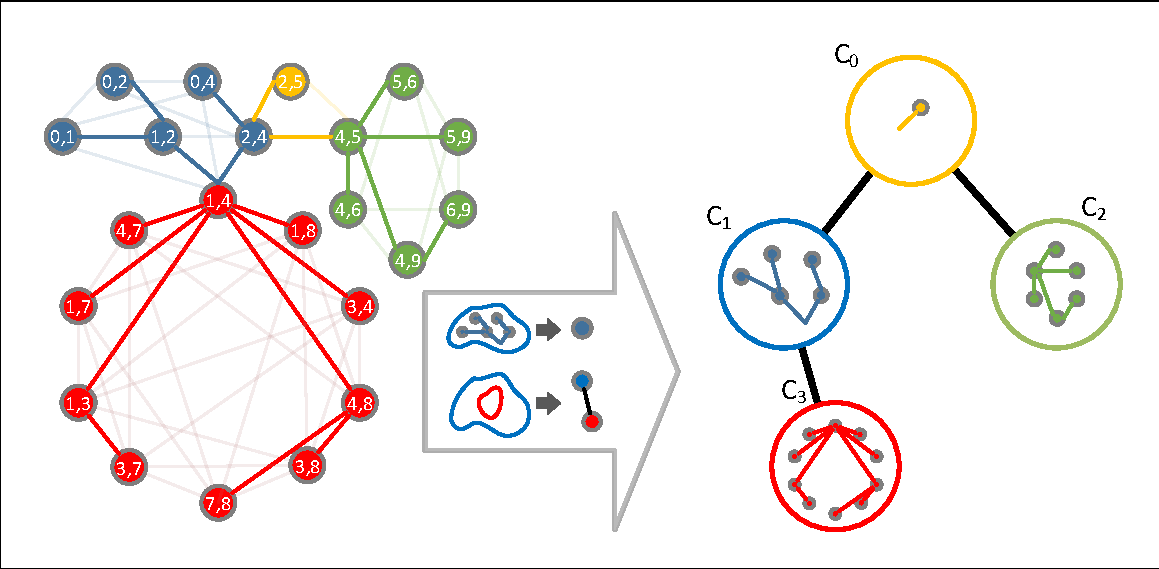
\includegraphics[width=0.8\linewidth, trim={0.6cm 0.6cm, 0.6cm, 0.6cm}, clip]{./figures/top_level.pdf}
		\vspace{-0.2cm}
    \caption{Construction of the \treeindex{} from the \inducedgraph{}. The graph on the left is an MST of the \inducedgraph{}. The graph on the right is the \treeindex{} having vertices that represent unique k-truss communities and edges that represent the containment relations between k-truss communities. The color of vertices shows the mapping between graphs.}
    \label{fig:top-level}
		\vspace{-0.1cm}
\end{figure}

~\\The top-level index is a super-graph whose vertices represent unique k-truss communities and edges represent containment relations between k-truss communities. We call this index structure the \treeindex{} and denote it as $G^c$. Based on the hierarchical property of k-truss \cite{cohen2008trusses}, \ie for $k \ge 2$, each $k$-truss is the subgraph of a ($k-1$)-truss, we have the formal definition of the \treeindex{} in \autoref{def:\treeindex{}}. We show an example of the \treeindex{} in \autoref{fig:top-level}.

\begin{Def}[\Treeindex{}]
The \treeindex{} $G^c$ is a weighted undirected graph that represents each k-truss community in the original graph $G^o$ by a vertex. $G^c$ has an edge $e^c$ connecting vertices $v^{c}_{1}, v^{c}_{2} \in G^{t}$ if and only if the following two conditions are met for their corresponding k-truss communities $C^{o}_{1}, C^{o}_{2} \in G^{o}$:
\begin{itemize}
	\item $C^{o}_{1}$ is a subgraph of $C^{o}_{2}$ or the other way around.
	\item We assume without loss of generality that $C^{o}_{1}$ is a subgraph of $C^{o}_{2}$, there is no $C^{o}_{3} \in G^{o}$ such that $C^{o}_{1}$ is a subgraph of $C^{o}_{3}$ and $C^{o}_{3}$ is a subgraph of $C^{o}_{2}$.
\end{itemize}
$G^c$ only has vertex weights, which represent the trussness of the corresponding k-truss communities.
\label{def:\treeindex{}}
\end{Def}

A key property of the \treeindex{} is that it is a forest. For the sake of space, we omit the proofs here. This property enable us to easily construct the \treeindex{} with a single breath first search (BFS) on the bottom-level index $G^m$. The traversal algorithm creates a tree in the \treeindex{} $G^c$ of each connected component in $G^m$. To construct a tree in $G^c$, the algorithm iteratively processes vertices in $G^m$ using the BFS and map vertices in $G^m$ to vertices in $G^c$. The map between a vertex $u^m \in G^m$ to a vertex $v^c \in G^c$ means the k-truss community represented by $v^c$ has the highest trussness among all k-truss communities that contains the edge represented by $u^m$. We store this mapping in a lookup table $H$. For example, in our example graph in \autoref{fig:example}, edge $1,4$ belongs to three k-truss communities denoted as $C_{0}, C_{1},$ and $C_{3}$ in \autoref{fig:top-level}. Since $C_{3}$ has the highest trussness of $5$, edge $1,4$ is mapped to $C_{3}$.

When the traversal algorithm reaches a vertex $v^{m}_{seed}$ belonging to a new connected component, it first creates a new super-vertex in $G^c$ and uses it as a starting point to build a new tree in $G^c$. Note that this starting point is not necessarily the root of the new tree. Thereafter, for an arbitrary vertex $u^m$ from the same connected component that has been discovered by the BFS, assuming its parent vertex during the search is $p^m$ (which has been mapped to $v^{c}_{p}$ already), $u^m$ will be mapped to an existing vertex or a new vertex in $G^c$ depending on the relations of the weight of the super-vertex $v^{c}_{p}$ and its ancestor in $G^c$, the weight of the edge $(p^m, u^m)$, and the weight of the vertex $u^m$. The detailed rule for the mapping can be found in Algorithm \ref{alg:\treeindex{}_construction}.

The reason we use weights of the edge $(p^m, u^m)$ between a vertex and its parent vertex as references when mapping a vertex of $G^m$ to $G^c$ is that edges in $G^m$ represents triangle adjacency in the original graph $G^o$. Since edge weight in $G^m$ represents minimum edge trussness in the corresponding triangle in $G^o$ and $G^m$ is a maximum spanning tree, the weight of edge $(p^m, u^m)$ limits the highest trussness of a k-truss community, to which $u^m$'s representing edge can belongs. 

%The procedure of mapping a vertex $u^m$ to a super vertex in $G^c$ can be divided in following two steps. First, start at $u^m$'s parent vertex $p^m$'s corresponding super vertex $v^{c}_{p}$, the algorithm exam ancestors of $v^{c}_{p}$ until it finds a super vertex with weight smaller than or equal to the weight of $(p^m, u^m)$ (line 8). This super vertex, which we reuse the symbol $v^{c}_{p}$, represents the community to which $u^m$ can triangle connect. Second, if $\tau_{e^m} = \tau_{u^m} = \tau_{v^{c}_{p}}$, we can directly map $u^m$ to $v^{c}_{p}$ (line 20). Otherwise, we need to create a new super vertex and either add it as a new child of $v^{c}_{p}$ (line 22) or insert it between $v^{c}_{p}$ and one of its existing child (line 11-12 and 14-16).

\begin{algorithm}
	\KwData{$G^{m}(V^{m},E^{m})$}
	\KwResult{$G^{c}(V^{c},E^{c})$, $H$}
	\SetKwProg{Fn}{function}{}{end}
	\SetKw{Continue}{continue}
	\SetKw{Break}{break}
	\BlankLine
	%$Q \gets \emptyset$, $bfsparent \gets \emptyset$, $unvisited \gets V^{m}$\;
	%\While{$unvisited \neq \emptyset$}{
		%$seed \gets$ $unvisited.pop()$, $Q \gets Q \bigcup seed$; \Comment{Seed for new tree.}\
	\For{each connected component $CC \in G^m$} {
		$v^{m}_{seed} \gets CC.pop()$\;
		create\_super\_vertex($seed$, $null$)\;
		%\While{$Q \neq \emptyset$}{
			%$u^m = Q.pop()$\;
			%\For{$v^m \in N_{u^m} \bigcup unvisited$}{
				%$Q \gets Q \bigcup v^{m}$, $bfsparent[v^{m}] \gets u^{m}$, $unvisited.remove(v^{m})$\;
			%}
		\For{$u^m \in$ BFS starting at $seed$} {
			$p^m \gets$ parent of $u^m$ in BFS\;
			$e^m \gets (u^m, p^m)$\;
			$v^{c}_{p} \gets H[p^m]$\;
			%$p^m \gets bfsparent[u^m]$, $e^m \gets (u^m, p^m)$, $v^{s}_{p} \gets H[p^m]$\;
			\lWhile{$\tau_{v^{c}_{p}} > \tau_{e^m}$}{
				%\uIf{$\tau_{v^{s}_{p}} > \tau_{e^m}$}{
					${v^{c}_{p}}^{\prime} \gets v^{c}_{p}$, $v^{c}_{p} \gets v^{c}_{p}.parent$
					%\Continue
			}
			%mapping $u^m$ based on $\tau_{v^{c}_{p}}$, $\tau_{e^m}$ and $\tau_{u^m}$
			\eIf{$\tau_{v^{c}_{p}} < \tau_{e^m}$}{
				\eIf{$\tau_{e^m} = \tau_{u^m}$}{
					$v^{c}_{u} \gets$ create\_super\_vertex($u$, $v^{c}_{p}$)\;
					${v^{c}_{p}}^{\prime}.parent \gets v^{c}_{u}$\;
				} {
					$v^{c}_{e} \gets$ create\_super\_vertex($e$, $v^{c}_{p}$)\; 
					$v^{c}_{u} \gets$ create\_super\_vertex($u$, $v^{c}_{e}$)\;
					${v^{c}_{p}}^{\prime}.parent \gets v^{c}_{e}$\;
				}
			} {
				\eIf{$\tau_{e^m} = \tau_{u^m}$}{
					$H[u^m] \gets v^{c}_{p}$\;
				} {
					$v^{c}_{u} \gets$ create\_super\_vertex($u$, $v^{c}_{p}$)\;
				}
			}
		}
	}
	\Return{$G^{c}(V^{c},E^{c})$, $H$}
	%\BlankLine
	%\Fn{create\_super\_vertex ($u^m$, $v^{c}_{p}$)}{
		%create $v^{c}_{u}$, $H[u^m] \gets v^{c}_{u}$\;
		%$v^{c}_{u}.parent \gets v^{c}_{p}$\;
		%$V^c \gets V^c \bigcup v^{c}_{u}$\;
		%\Return{$C_u$}
	%}
	\caption{Top Level Index Construction}
	\label{alg:\treeindex{}_construction}
\end{algorithm}

For each vertex of $G^m$, searching the ancestor super-vertex in $G^c$ of its parent vertex in $G^m$ takes $O(k_{max})$ time, where $k_{max}$ is the highest trussness of k-truss communities in $G^o$. Since the index construction process is a BFS on a maximum spanning tree with $O(|E^o|)$ vertices, the total construction time is $O(k_{max}|E^o|)$. As each vertex in $G^c$ represents a k-truss community in $G^o$, and $G^c$ is a forest, the algorithm takes $O(|C^o|)$ space and the index size is $O(|C^o|)$, where $|C^o|$ is the number of communities in $G^o$. 
%
%\begin{figure}[ht]
    %\centering
    %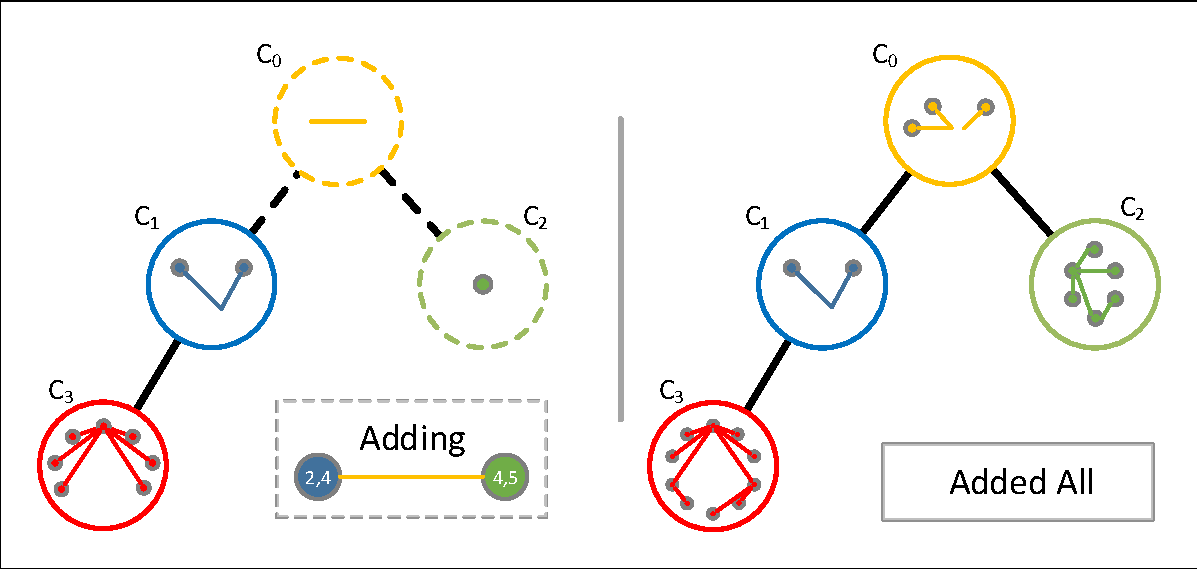
\includegraphics[width=\linewidth]{./figures/tree_index.pdf}
    %\caption{An example \treeindex{	} of the \inducedgraph{} in \autoref{fig:\inducedgraph{}}}
    %\label{fig:\treeindex{}}
%\end{figure}
%
%An example is shown in \autoref{fig:\treeindex{}}